\section{Computation and dynamics}



%%%%%%%%%%%%%%%%%%%%%%%%%%%%%%%%%%%%%%%%%%%%%%%%%%%%%%%%%%
\begin{frame}[label=ladila]{The criticality view I}
 \begin{center}
  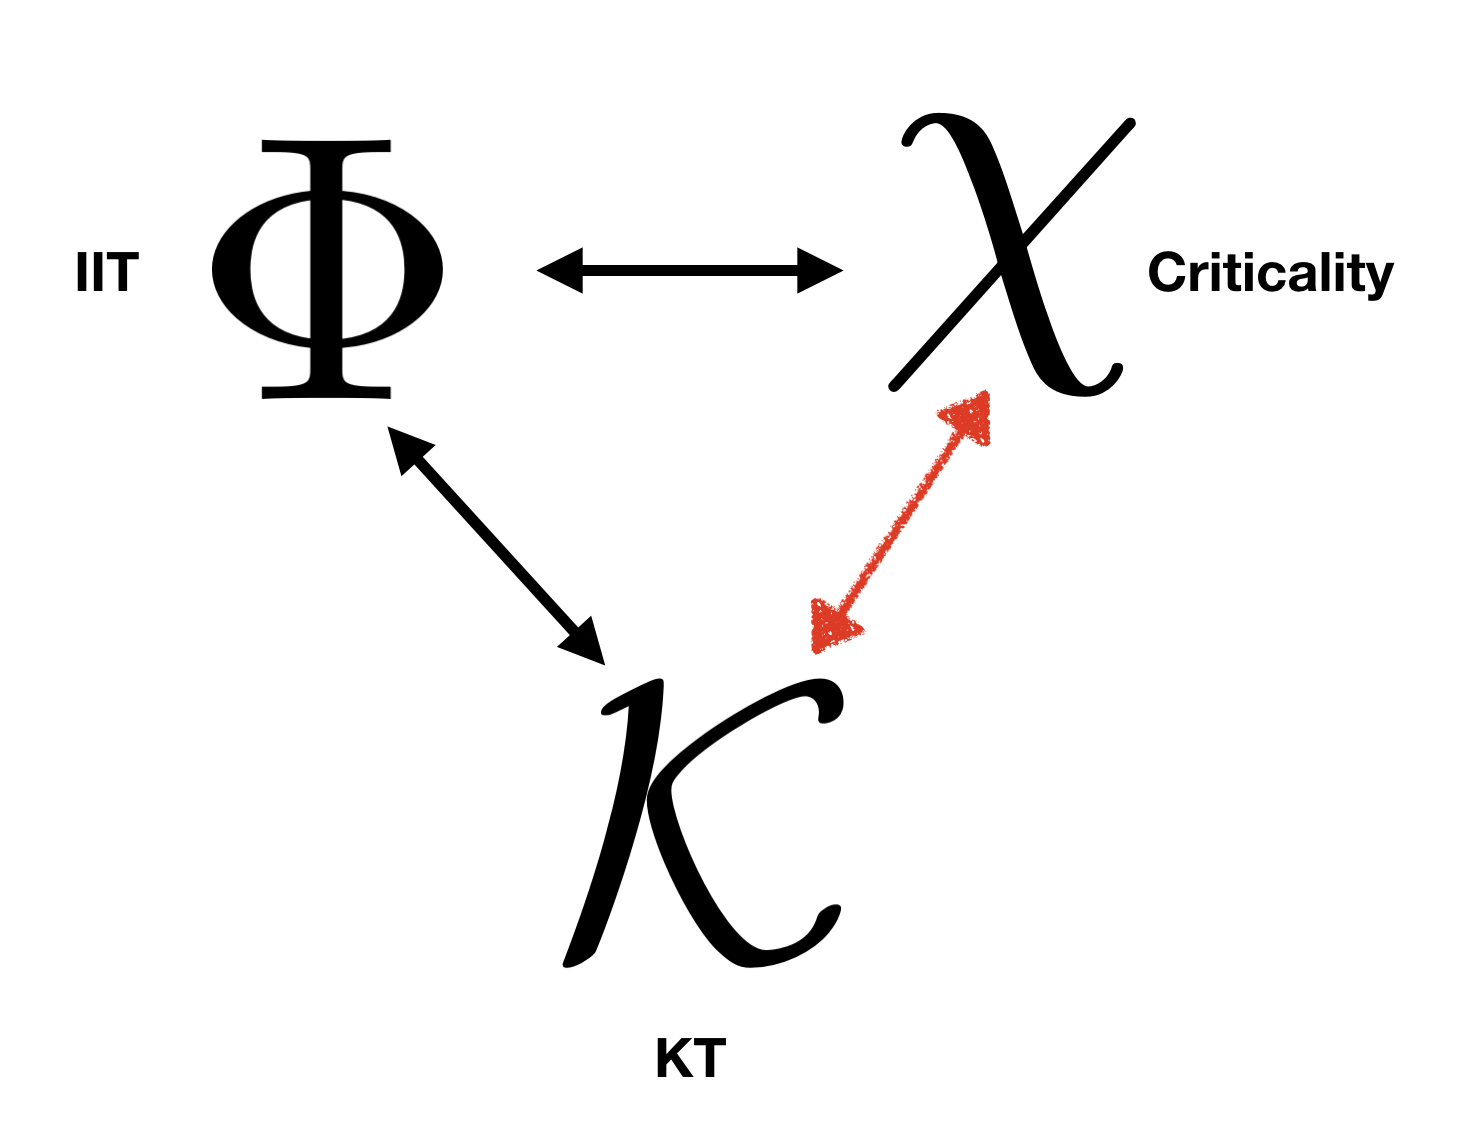
\includegraphics[height=8cm]{img/KUF.png}
  \end{center}
\end{frame}


%%%%%%%%%%%%%%%%%%%%%%%%%%%%%%%%%%%%%%%%%%%%%%%%%%%%%%%%%%
\begin{frame}[label=ladila]{The criticality view II}
 Computation  in Nature is carried out by dynamical systems with very large degrees of freedom.  \vfill
 
  Brains operate close to such critical boundaries consistent with the notion of self-organized criticality (SOC) \citep{Bak1988,Chialvo:2004aa,Cocchi2017,Carhart2018,Deco2021}. \vfill
  
  Altered state of consciousness appear to move the brain away or towards criticality \citep{CarhartHarris2019,Ruffini:2022ac}. %Ising temperature under LSD increases (Ruffini et al in prep).  
  \vfill
  
  KT and criticality theory:  Algorithmic agents (dynamical systems instantiating  compressive models of  data that exhibits regularities/symmetries)  must have special properties.  What are they?\vfill
 
  \end{frame}
  
  %%%%%%%%%%%%%%%%%%%%%%%%%%%%%%%%%%%%%%%%%%%%%%%%%%%%%%%%%%
  \begin{frame}[label=ladila]{The criticality view III}
  Recall the movie of a moving hand in empty space, $y(t) = f(\theta(t))$. %, where $y(t)$ represents the sequences of images of the hand as a function of parameters $\theta(t)$.
  \vfill
  
  Although $y$ may be embedded in a very high dimensional space, its dimension is actually very small if the set of parameters $\theta$ controlling the hand function is small.\vfill
  
The state of a dynamical system generating frames of the moving hand, regardless of how large its natural space is  (e.g.,   large number of neurons) must also lie in a low dimensional subspace, a {\bf reduced manifold}. How?  \vfill
  
   Criticality: near criticality (Re[$\lambda$]$\sim0$) the dynamics of complex systems collapse to low dimensional manifolds   \citep{Jirsa2020,Jirsa2022}---constrained dynamics. \vfill
   
   Symmetry: in a Hamiltonian dynamical system where $g = y(t)-f(\theta(t)) = 0$  (the constraint),  Noether's theorem states that  $H$ is invariant under the group of symmetries generated by $g$  \citep{Dirac2001-gi,Jose1998-qy}). 

\end{frame}

%%%%%%%%%%%%%%%%%%%%%%%%%%%%%%%%%%%%%%%%%%%%%%%%%%%%%%%%%%
\begin{frame}[label=ladila]{The criticality view IV---the center manifold}
Trajectory of representation of hand in reduced manifold. 
 \begin{center}
  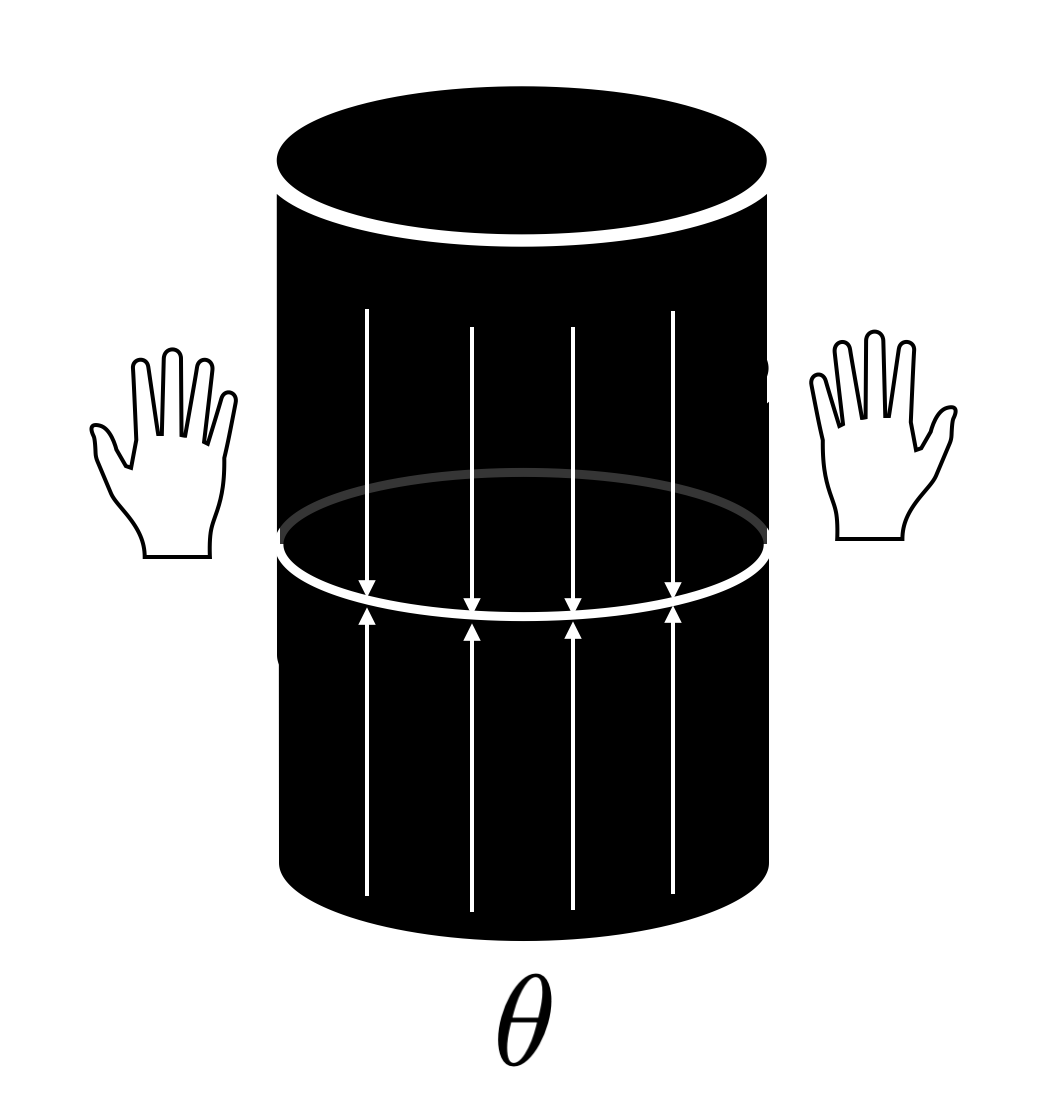
\includegraphics[height=6cm]{img/cylinder.png}
  \end{center}


\end{frame}



%%%%%%%%%%%%%%%%%%%%%%%%%%%%%%%%%%%%%%%%%%%%%%%%%%%%%%%%%%
\begin{frame}[label=ladila]{The criticality view V}

   Structure/symmetry in data, the collapse of dynamics to low-dimensional spaces, criticality (maximal information flow, power laws, long time scales and enhanced susceptibility),  \K and \SEP are thus deeply connected. \vfill 
   
The  manifold structure of the reduced dynamics together with  $\mathcal M$ provide, respectively, metrics on the simplicity of the  models and the amount of algorithmic information captured.  \vfill




The agent-world-lock loop---which tracks world   data---keeps dynamics on the reduced manifold (\SEP!). Psychedelics, meditation, sensory deprivation, neuropsychiatric disorders, may ``lift'' up the enslaved dynamics.
\end{frame}

